\section{Scalar}
For scalar values are a few functions available

\subsection{Multiplication and Rightshift}
Represents $ a \multiplication b $ with a right shift about \textit{r}. This becomes close to
\begin{equation}
2^{-r} a \multiplication b
\end{equation}
but it is not the same.
\inHfile{INT\_MULT\_RSHIFT(a, b, r)}{pprz\_algebra\_int}

\subsection{$\sqrt x$ Squareroot}
Calculates the squareroot $y = \sqrt x$. The function uses the Babylonian method.
\begin{equation}
y_{n+1} = \frac 1 2 \left( y_n + \frac{x}{y_n} \right)
\end{equation}
\inHfile{INT32\_SQRT(out,in)}{pprz\_algebra\_int}

\subsection{atan2() 4-quadrant arctangent}
Calculates the 4-quadrant arctangent of two values, x and y:
\begin{equation}
a = atan2(y,x)
\end{equation}
The function uses a trick, which is desribed in detail at
\begin{itemize}
\item http://www.dspguru.com/comp.dsp/tricks/alg/fxdatan2.htm
\end{itemize}
In short:


\begin{figure}[h!]
	\centering
	\begin{tabular}{ccc}
	
		\begin{minipage}{4cm}
		\centering
		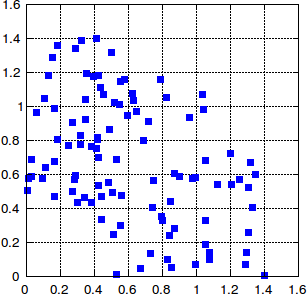
\includegraphics[width=4cm]{xyvalues}
		\end{minipage}
	&
		\begin{minipage}{4cm}
		\centering
		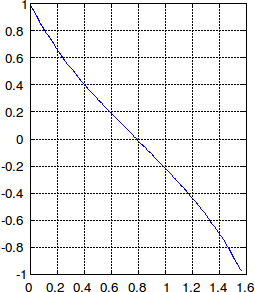
\includegraphics[width=4cm]{ratiofunction}
		\end{minipage}
	&
		\begin{minipage}{5cm}
		\centering
		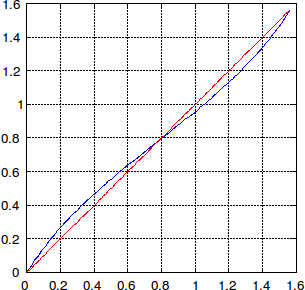
\includegraphics[width=4cm]{atan2_alternate}
		\end{minipage}
	\\
		(a) x/y-values  &
		(b) ratio function & 
		(c) comparison of the result (blue)
	\\
		& & and the real value (red)
	\end{tabular}
	
	\caption{alternate atan2 function} \label{alternate atan2 function}
\end{figure}

If you have a set of x/y values (figure \ref{alternate atan2 function}a), you can compute the ratio (figure \ref{alternate atan2 function}b) of them:
\begin{equation}
	r = \frac{x+y}{x-y}
\end{equation}
and transform this ratio very close to the real values (figure \ref{alternate atan2 function}c) using
\begin{equation}
	\alpha = \tfrac \pi 4 (1-r)
\end{equation}
or (more accurate) using
\begin{equation}
	\alpha_2 = 0.1963 \multiplication r^3 -0.9817 \multiplication r + \tfrac \pi 4
\end{equation}
\inHfile{INT32\_ATAN2(a, y, x)}{pprz\_algebra\_int}
\inHfile{INT32\_ATAN2\_2(a, y, x)}{pprz\_algebra\_int}